\begin{flushleft}
	\section{\textcolor{cyan}{Réalisation du système de télésurveillance : }}
	    	\subsection{\textcolor{green}{Circuits électriques et prototype :}}
		    
	    \begin{figure}[h]
	    \centering
	    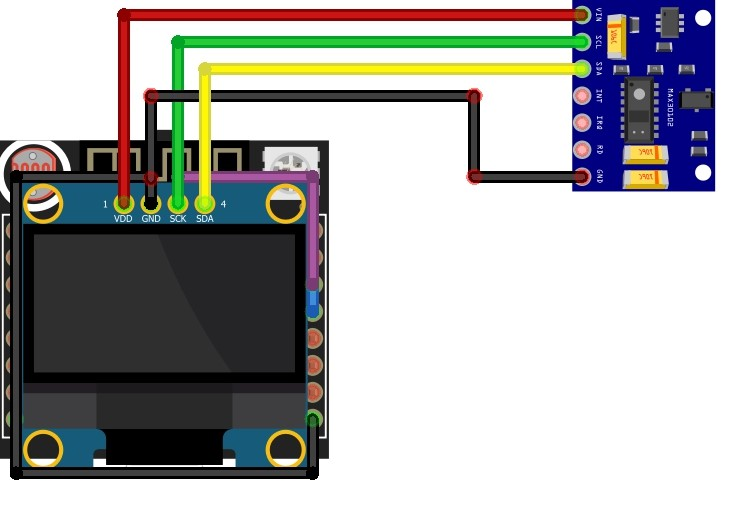
\includegraphics{chapitres/images/Systeme-de-telesurveillance_bb2.jpg}
		\end{figure}
		\begin{figure}[h]
		\centering
		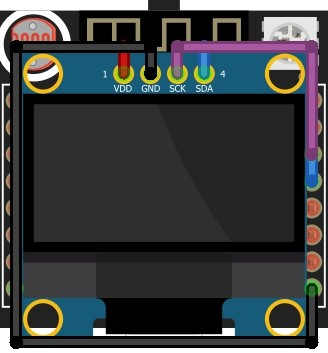
\includegraphics{chapitres/images/Systeme-de-telesurveillance_bb.jpg}
		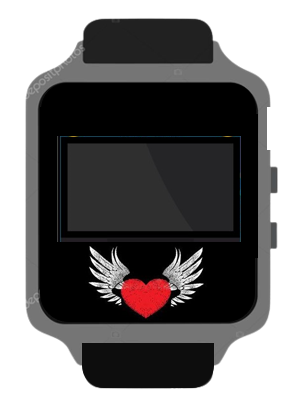
\includegraphics{chapitres/images/SmartWath.PNG}
		\caption{Circuits électriques et prototype}
		\label{fig:labelname}
	\end{figure}
\newpage
	\subsection{\textcolor{green}{Connection de l'ESP8266 à AWS IoT Core :}}
	La connexion de l'ESP8266 à AWS IoT Core implique plusieurs étapes. Voici un aperçu des étapes à suivre:
	
	1. Créer un compte AWS: Si vous n'avez pas de compte AWS, vous devez d'abord en créer un. Vous pouvez vous inscrire à l'aide de ce lien: https://aws.amazon.com/fr/free/.
	
	2. Créer un groupe de sécurité: Un groupe de sécurité permet de spécifier les règles de trafic entrant et sortant pour les instances EC2. Pour créer un groupe de sécurité, vous devez vous rendre dans le tableau de bord AWS et sélectionner l'option "Groupe de sécurité" dans la section "Sécurité, Identité et Conformité".
	
	3. Créer un certificat: Pour communiquer avec AWS IoT Core, vous devez créer un certificat et une clé privée. Vous pouvez générer ces éléments à l'aide du kit de développement logiciel AWS IoT (SDK). Vous pouvez télécharger le SDK ici: https://aws.amazon.com/fr/iot-sdk/.
	
	4 Configurer l'ESP8266: Vous devez configurer l'ESP8266 pour qu'il puisse communiquer avec AWS IoT Core. Pour ce faire, vous pouvez utiliser l'IDE Arduino et la bibliothèque AWS IoT. Vous pouvez télécharger la bibliothèque AWS IoT ici: https://github.com/aws/aws-iot-device-sdk-arduino-yt.
	
	5. Publier des messages: Une fois que votre ESP8266 est configuré, vous pouvez publier des messages sur AWS IoT Core. Vous pouvez le faire en utilisant la méthode "publish" de la bibliothèque AWS IoT.
		
		\begin{figure}[h]
			\centering
			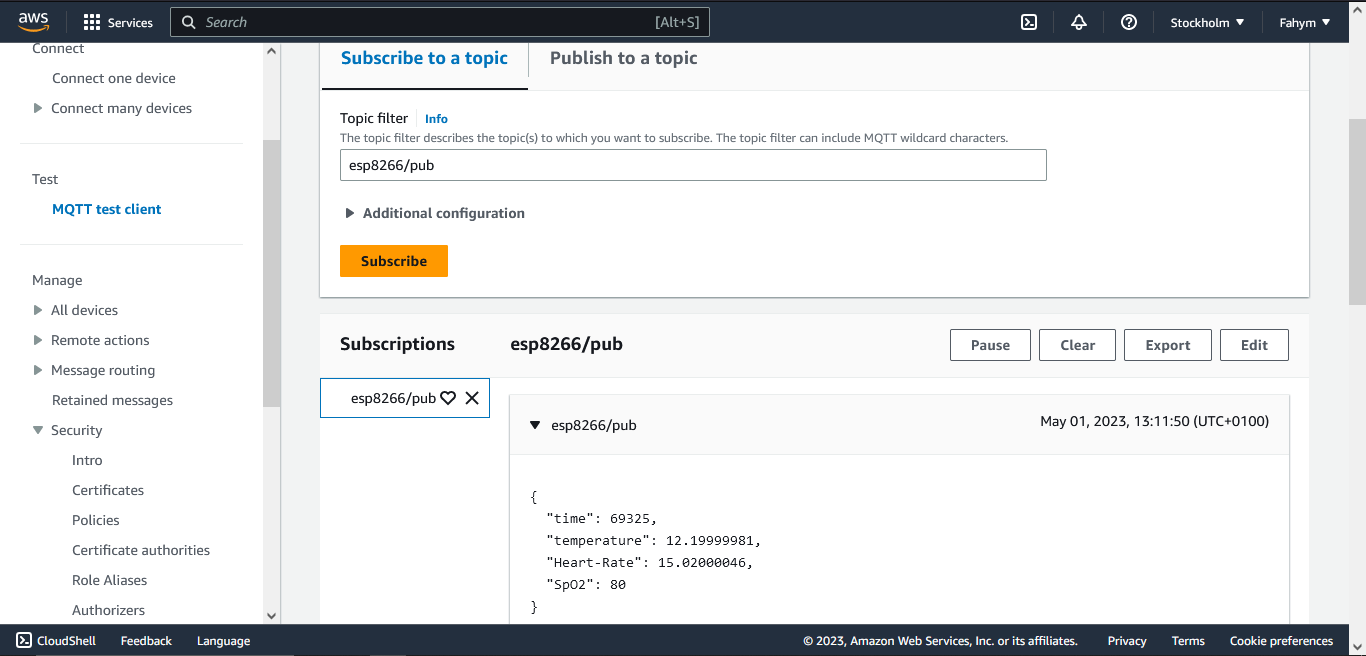
\includegraphics[width=0.9\textwidth]{chapitres/images/aws2.PNG}
			\caption{Connection de l'ESP8266 à AWS IoT Core}
			\label{fig:labelname}
		\end{figure}
	
	\newpage
	\subsection{\textcolor{green}{Réalisation finale du prototype :}}
	
			
			\begin{figure}[h]
				\centering
				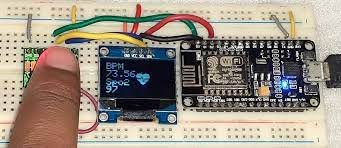
\includegraphics[width=0.8\textwidth]{chapitres/images/Prototyp2.jpg}
				\caption{Prototype finale}
				\label{fig:labelname}
			\end{figure}
	\newpage
\end{flushleft}